\documentclass[12pt]{article}
\usepackage[utf8]{inputenc}
\usepackage{geometry}
\geometry{left=3cm,right=3cm,top=2cm,bottom=2cm}
\usepackage{graphicx}
\usepackage{hyperref} % Essential for hyperlinks
\usepackage{titlesec} % Customize sections
\titleformat{\section}{\normalfont\Large\bfseries}{\thesection}{1em}{}
\usepackage{amsmath}
\usepackage{amsfonts}
\usepackage{changepage}
\usepackage[backend=biber, style=apa, sorting=nyt]{biblatex} % For bibliography
\addbibresource{sn-bibliography.bib} % Your bibliography file
\usepackage{booktabs} % For formal 
\usepackage{ragged2e}
\usepackage{microtype}
\usepackage{multirow}
%\usepackage{multicol}

% Remove the fancyhdr settings if you're not using them
% \usepackage{fancyhdr} % Enhanced header and footer
% \pagestyle{fancy}
% \fancyhf{}
% \rhead{\thepage}
% \lhead{\leftmark}
% \renewcommand{\headrulewidth}{0.4pt}


%% \usepackage{fancyhdr} % Enhanced header and footer
%% \pagestyle{fancy}
%% \fancyhf{}
%% \rhead{\thepage}
%% \lhead{\leftmark}
%% \renewcommand{\headrulewidth}{0.4pt}


\small
\title{\textbf{Optimizing KGQA Systems: A Systematic Comparative Study of Negative Sampling Strategies in KGE Models}} % Title is explicitly bolded

\author{%
    \text{Medhasweta Sen}\textsuperscript{1}, \href{mailto:msen22@gwu.edu}{msen22@gwu.edu} \\
    \text{Nina Ebensperger}\textsuperscript{1}, \href{mailto:nebensperger85@gwu.edu}{nebensperger85@gwu.edu} \\
    \text{Nayaeun Kwon}\textsuperscript{1}, \href{mailto:nkwon@gwu.edu}{nkwon@gwu.edu} \\
    \text{Dr. Amir Jafari}\textsuperscript{1}, \href{mailto:ajafari@gwu.edu}{ajafari@gwu.edu} \\
    \textsuperscript{1}Department of Data Science, \\
    The George Washington University, \\
    Washington DC, USA
}
\date{}

\begin{document}
\raggedright

\maketitle

\begin{abstract}
Knowledge Graph Question Answering (KGQA) systems facilitate intuitive interactions with structured knowledge bases by interpreting and answering natural language queries. The efficacy of these systems largely hinges on the robustness of the underlying Knowledge Graph Embeddings (KGEs), which capture semantic relationships between entities. This paper explores the impact of various negative sampling techniques on the performance of different KGE models in the context of KGQA. We experiment with multiple KGE models, including DistMult, and ComplEx, employing diverse negative sampling strategies such as Uniform, Random Corrupt, and Batch Negative Sampling. Our evaluation, conducted across several benchmark knowledge graphs, focuses on both the quality of the embeddings and the downstream KGQA performance. The results highlight significant variations in accuracy and response time, underscoring the critical role of negative sampling in enhancing KGQA systems. This study aims to provide insights into optimizing KGQA frameworks by tailoring the embedding generation process, thereby paving the way for more effective and efficient question-answering capabilities over knowledge graphs.

\end{abstract}
%\begin{multicols}{2}
\section{Introduction}

Knowledge Graph Question Answering (KGQA) is designed to answer natural language questions by utilizing structured facts stored in knowledge graphs. Despite its potential, KGQA faces significant challenges, primarily in retrieving related facts and leveraging the reasoning capabilities of knowledge graphs for question answering. To address these challenges, recent advancements have integrated Large Language Models (LLMs) to enhance the interaction between natural language queries and structured knowledge. This approach, known as LLM-augmented KG Question Answering, utilizes LLMs in two main capacities: as entity/relation extractors and as answer reasoners. These advancements and the foundational concept of LLM-augmented KGQA are detailed extensively in the work of Pan et al. \parencite{Pan2023UnifyingLL}.


As entity/relation extractors, LLMs are adept at identifying relevant entities and relationships within natural language questions, thereby facilitating the retrieval of pertinent facts from knowledge graphs. This application has been demonstrated to significantly improve performance over traditional methods, with notable implementations including classifiers for relation prediction and frameworks for detecting mentioned entities and relations.

In their role as answer reasoners, LLMs leverage the extracted information to reason over and generate answers directly from the knowledge graphs. This process often involves encoding questions alongside candidate answers and facts, and using the LLM's powerful comprehension capabilities to predict the most likely answers. Innovations such as dynamic reasoning models and knowledge interaction layers further enhance this capability, allowing for more effective and nuanced reasoning over complex queries.

Overall, LLM-augmented KGQA represents a transformative approach that merges the deep understanding of language provided by LLMs with the structured reasoning capabilities of knowledge graphs, aiming to provide more accurate and contextually relevant answers to natural language questions.

In this paper, we explore the utilization of LLMs as encoders within the KGQA framework, focusing on enhancing knowledge graph embeddings (KGE) through innovative negative sampling techniques. Our goal is to refine the accuracy and efficiency of KGQA systems, pushing the boundaries of how effectively these models can interpret and process complex queries in a structured knowledge environment.
% \end{multicols}

\begin{figure}[!ht] % 'h!' places the figure here, within your text
  \centering % Centers the figure
  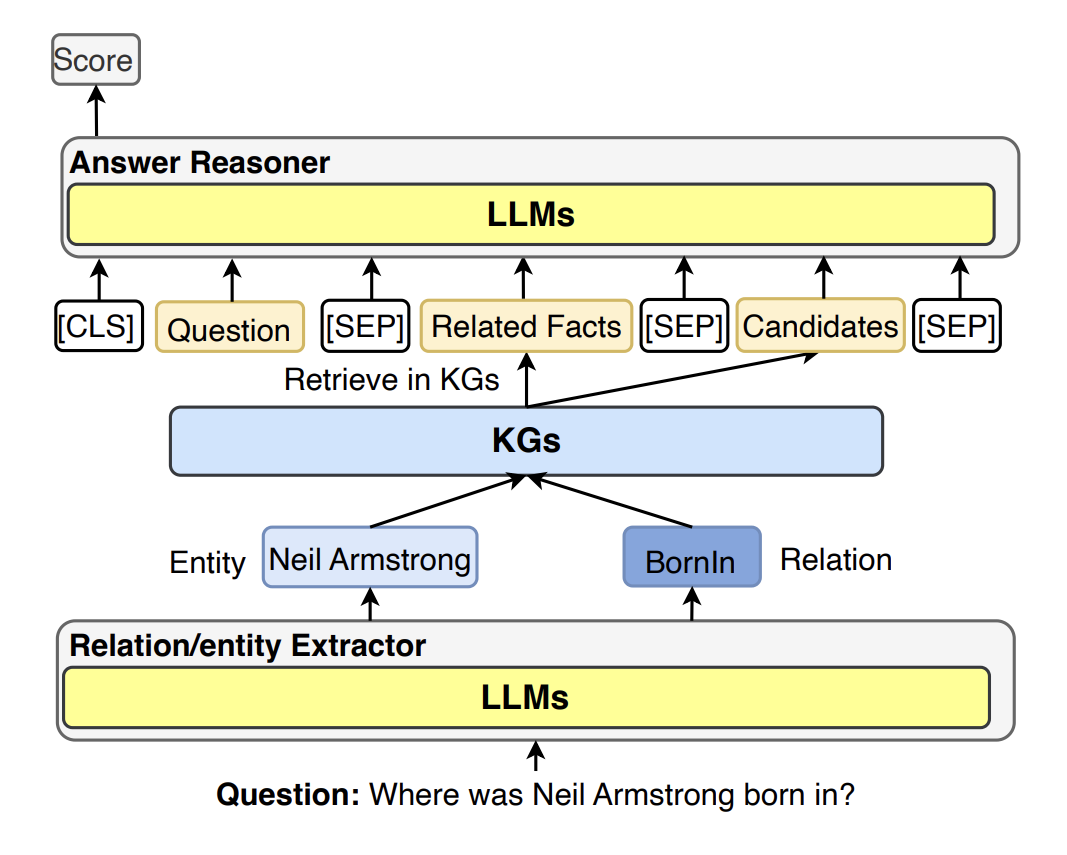
\includegraphics[width=0.8\textwidth]{introduction_img.png} % Adjust the width to 80% of the text width
  \caption{The general framework of applying LLMs for knowledge graph
question answering (KGQA)(figure from \textcite{Pan2023UnifyingLL}
} % Caption for the figure} % Caption for the figure
  \label{fig:introduction_img} % Label for referencing this figure
\end{figure}

\section{Related Work}
This section reviews significant advancements in Knowledge Graph Question Answering (KGQA), focusing on the integration of Large Language Models (LLMs) and Knowledge Graph Embeddings (KGEs) and evolving KGE computation using various Techniques.

\subsection{Knowledge Graph Embeddings Computation}

\subsubsection{ComplEx}
\textcite{trouillon2016complex}
 introduced the ComplEx model, which employs complex-valued embeddings for link prediction in knowledge bases. The primary innovation of the ComplEx model is its use of complex numbers to represent entities and relations in a knowledge graph, enabling the capture of both symmetric and antisymmetric relations effectively.

The approach centers around the Hermitian dot product, defined for complex vectors $\mathbf{u}$ and $\mathbf{v}$ as $\langle \mathbf{u}, \mathbf{v} \rangle = \mathbf{u}^H \mathbf{v}$, where $\mathbf{u}^H$ is the conjugate transpose of $\mathbf{u}$. In the context of knowledge graphs, if we let $\mathbf{e}_s, \mathbf{e}_o \in \mathbb{C}^K$ be the embeddings for a subject $s$ and an object $o$, and $\mathbf{r} \in \mathbb{C}^K$ the embedding for the relation, the scoring function for a fact $(s, r, o)$ is given by:
\[
\phi(s, r, o) = \text{Re}(\langle \mathbf{r}, \mathbf{e}_s, \overline{\mathbf{e}_o} \rangle)
\]
where $\overline{\mathbf{e}_o}$ is the complex conjugate of $\mathbf{e}_o$, and $\text{Re}(z)$ denotes the real part of the complex number $z$.

This model is particularly adept at modeling antisymmetric relations due to the non-commutative property of the Hermitian product. It simplifies to $\text{Re}(\mathbf{r}^T (\mathbf{e}_s \odot \overline{\mathbf{e}_o}))$, where $\odot$ denotes the element-wise product. This formulation allows the ComplEx model to capture intricate relational patterns while remaining computationally efficient, as the model's complexity is linear with respect to the number of entities and relations.

\sloppy
The authors evaluated ComplEx on standard knowledge graph benchmarks such as FB15K and WN18, demonstrating its superiority over several baseline models including DistMult and HolE. The model excelled particularly in scenarios involving complex relational data with inherent asymmetries, showcasing higher Mean Reciprocal Rank (MRR) and Hits@K metrics compared to its counterparts.
\sloppy

\subsubsection{DistMult}
DistMult \textcite{yang2015embedding} presents a unified learning framework that generalizes several existing embedding models, including Neural Tensor Network (NTN) and TransE \textcite{bordes2013translating}, for knowledge base embeddings. The authors propose embedding entities and relations using a neural-embedding approach, where entities are represented as low-dimensional vectors, and relations are modeled as bilinear and/or linear mapping functions. This approach is particularly adept at addressing scalability and reasoning within large knowledge bases.

\textcite{yang2015embedding}. demonstrate that a simplified bilinear model, DistMult, can outperform complex models on tasks like link prediction. DistMult represents relations using a diagonal matrix in a bilinear scoring function:

\begin{equation}
s(e_1, r, e_2) = \mathbf{e_1}^\top \mathbf{M}_r \mathbf{e_2}
\end{equation}

where $\mathbf{e_1}$ and $\mathbf{e_2}$ are the embeddings of the entities, and $\mathbf{M}_r$ is the diagonal matrix specific to relation $r$. This formulation is advantageous due to its simplicity and the reduced number of parameters, leading to faster computation and less overfitting.

Moreover, the authors introduce an innovative approach for mining logical rules from the embeddings, enhancing the interpretability of the embeddings and supporting compositional reasoning. They demonstrate that embeddings learned through the DistMult model are particularly effective at capturing the compositional semantics of relations, which can be articulated as:

\begin{equation}
\mathbf{M}_{r1} \mathbf{M}_{r2} \approx \mathbf{M}_{r3}
\end{equation}

indicating that the composition of relations $r1$ and $r2$ can approximate relation $r3$. This property is key for rule mining and was shown to outperform traditional rule mining methods. Their empirical results on datasets such as Freebase highlight the model's robustness and its capability to improve link prediction accuracy significantly.

\textcite{yang2015embedding}'s work contributes substantially to the field by simplifying the modeling of entities and relations while maintaining or enhancing performance on key tasks, such as link prediction and rule extraction. Their methodological innovations provide a basis for further exploration into how knowledge graph embeddings can be effectively integrated with LLMs for KGQA.

\subsection{Question Answering over Knowledge Graphs}
In the realm of Knowledge Graph Question Answering (KGQA), the quest for efficient and accurate answers has led to the integration of various sophisticated techniques, primarily focusing on the use of Knowledge Graph Embeddings (KGEs) and Large Language Models (LLMs). The evolution of these methods reflects a significant transition from basic embeddings to more complex, multi-dimensional approaches capable of handling nuanced, multi-hop queries.

\subsubsection{Early Developments}
Historically, KGQA systems relied heavily on embedding models like TransE \textcite{bordes2013translating}, which simplified entities and relations into low-dimensional vectors. However, such models often struggled with multi-hop question answering due to their limited capacity to encapsulate complex relational paths. To overcome these limitations, advancements such as the ComplEx model \textcite{trouillon2016complex} introduced embeddings in complex vector spaces, enhancing the system's ability to interpret and link multiple relational entities dynamically.

\subsubsection{Enhancements Through Sub-Graph Extraction}
Further refinements in KGQA saw the introduction of methods aimed at extracting relevant sub-graphs from the knowledge graph to form answer hypotheses \parencite{yih2015semantic, bao2016constraint}. This approach allowed for a more targeted search space, reducing computational overhead and improving accuracy by focusing on potentially relevant portions of the graph. Moreover, the use of Memory Networks and other neural architectures began to emerge, facilitating the learning of more intricate embeddings directly from the knowledge graph's structure.

\subsubsection{Integration of Textual Data}
A pivotal advancement in the field was the integration of textual data as an auxiliary source of information to complement the knowledge graphs, especially beneficial for handling incomplete graphs (Sun et al., 2018, 2019a). This dual-source approach added a layer of complexity but significantly enriched the context available for answering more complex questions.

\subsubsection{The Embed-KGQA Model}
The Embed-KGQA model \parencite{saxena-etal-2020-improving} represents a culmination of these developments, incorporating multi-dimensional embeddings and advanced neural techniques to enhance the question-answering capabilities of KG systems. The model comprises several key components from \textcite{Pan2023UnifyingLL}.:
\sloppy
\begin{itemize}
    \item \textbf{KG Embedding Module:} Utilizes models like ComplEx to embed entities and relations in a complex space, facilitating a richer representation that is beneficial for capturing the nuances of various relational patterns.
    \item \textbf{Question Embedding Module:} Employs advanced language models, such as RoBERTa, to convert natural language questions into embeddings that accurately reflect their semantic and contextual nuances.
    \item \textbf{Answer Selection Module:} Integrates the embeddings from the KG and the question to predict the most accurate answers, using sophisticated scoring functions and relation matching techniques to enhance accuracy and efficiency, particularly in extensive knowledge graphs.

\end{itemize}
\fussy
\subsubsection{Challenges and Future Directions:} Despite these advancements, challenges remain, particularly in the scalability of these models and their ability to handle dynamically changing knowledge bases. Future research directions may include more adaptive models that can update their embeddings in real-time and the integration of more granular linguistic features to further refine the accuracy of KGQA systems \parencite{Pan2023UnifyingLL}.

\section{Knowledge Graphs and Knowledge Graph Embeddings}
In this section we will explain Knowledge Graphs and Embeddings based on the research of \textcite{Pan2023UnifyingLL}. 

\subsection{Knowledge Graphs}

\begin{figure}[!ht] % 'h!' places the figure here, within your text
  \centering % Centers the figure
  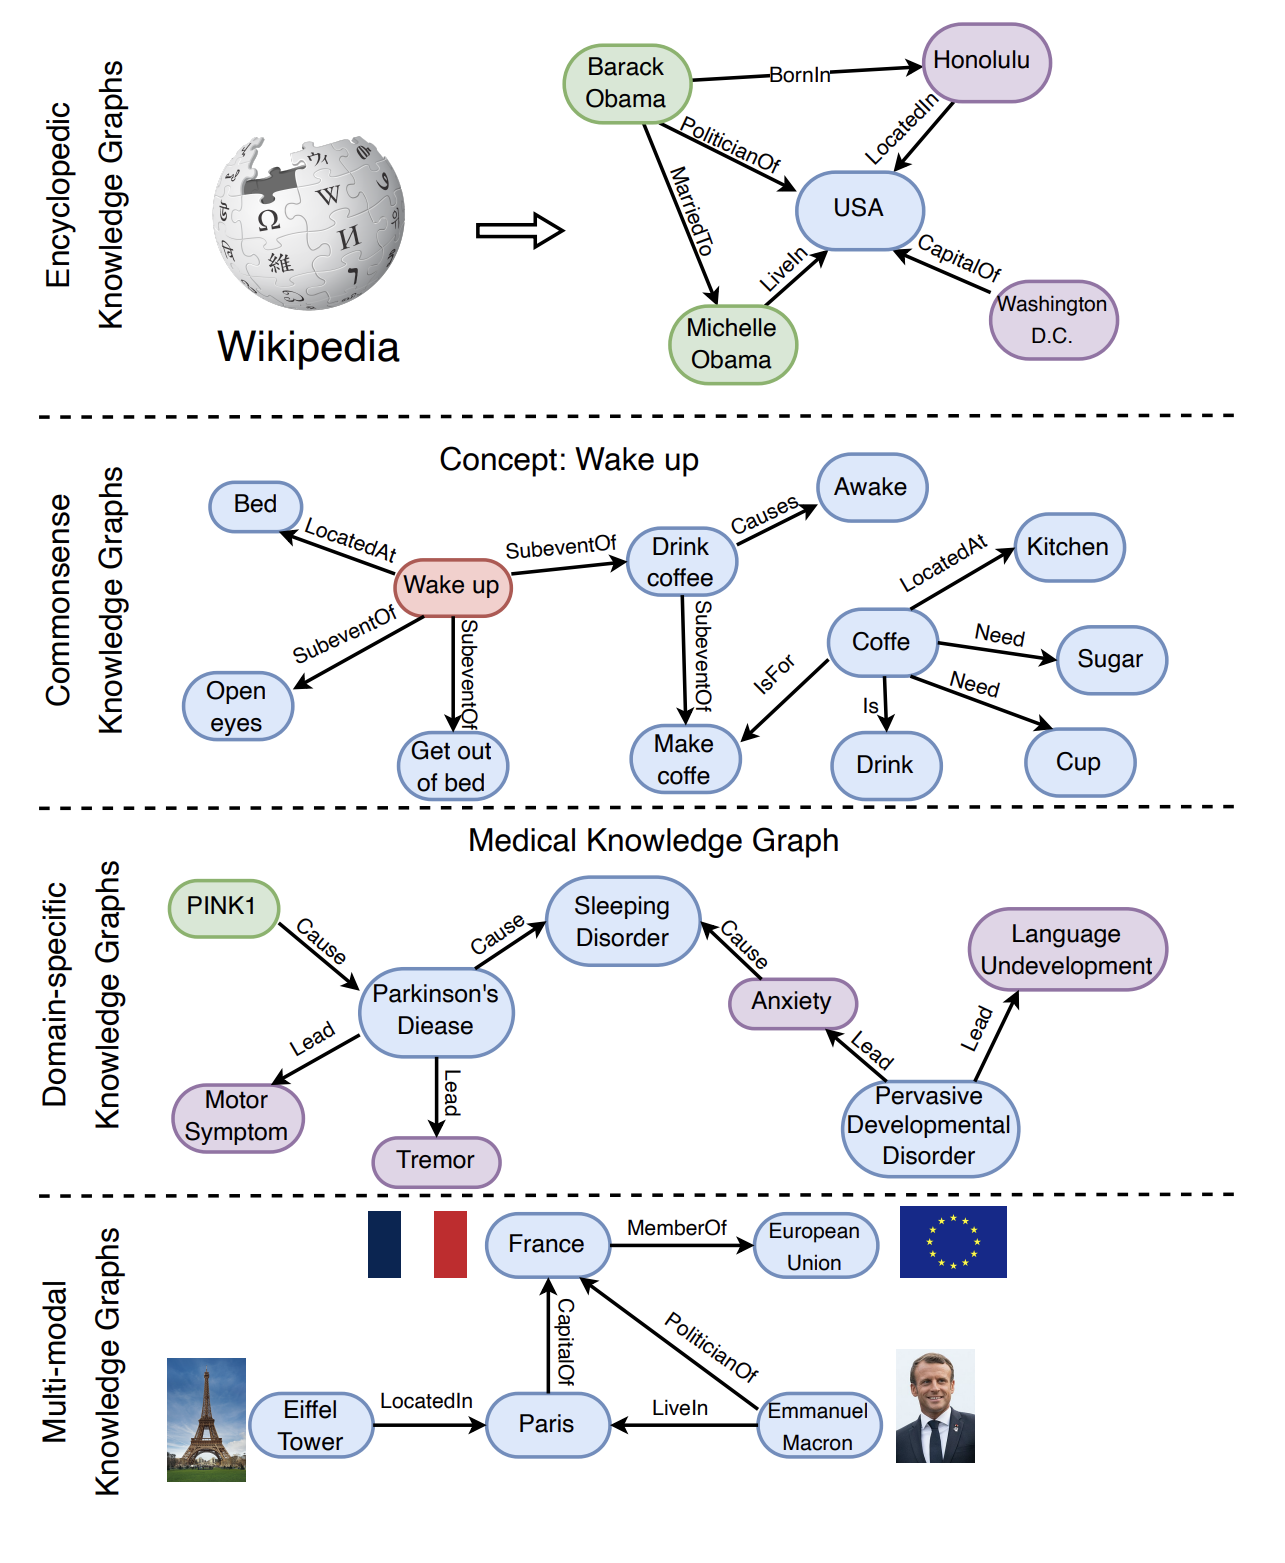
\includegraphics[width=0.8\textwidth]{KG_img.png} % Adjust the width to 80% of the text width
  \caption{Examples of different categories’ knowledge graphs, i.e., encyclopedic KGs, commonsense KGs, domain-specific KGs, and multi-modal KGs (figure from \textcite{Pan2023UnifyingLL}
} % Caption for the figure
  \label{fig:KG_img} % Label for referencing this figure
\end{figure}

Knowledge graphs (KGs) have become foundational in structuring and harnessing the complex webs of data across various scientific, technological, and practical domains. Defined fundamentally as a collection of triples 
\[
\text{KG} = \{(h, r, t) \subseteq \mathcal{E} \times \mathcal{R} \times \mathcal{E}\},
\]
where \(\mathcal{E}\) denotes entities and \(\mathcal{R}\) denotes relations between these entities, knowledge graphs enable the storage of structured knowledge in a semantically rich format. This structured knowledge supports advanced data integration, querying, and analysis capabilities, which are crucial for developing intelligent systems that understand and manipulate large datasets effectively.

The existing literature categorizes knowledge graphs into four distinct types based on the nature of the stored information: 1) Encyclopedic KGs, 2) Commonsense KGs, 3) Domain-specific KGs, and 4) Multimodal KGs. Each category serves different purposes and comes with unique characteristics. Encyclopedic knowledge graphs, such as Wikidata, Freebase, and Dbpedia, compile general knowledge from extensive sources and are instrumental in providing broad informational coverage. Commonsense knowledge graphs, like ConceptNet and ATOMIC, encode everyday knowledge about objects and their interactions, facilitating machines in understanding daily human concepts. Further, domain-specific knowledge graphs focus on specialized fields such as medicine or finance, exemplified by UMLS and various finance-specific KGs. These graphs prioritize precision and domain-\hspace{0pt}relevance over the breadth of information. Lastly, multimodal knowledge graphs, such as IMGpedia and MMKG, integrate data from various modalities, including text, images, and videos, enhancing the richness of the data representation and supporting complex applications like visual question answering and multimedia recommendations.

\subsection{Knowledge Graphs Embeddings}

While knowledge graphs (KGs) are powerful tools for representing and querying relationships between entities, their structural form alone can sometimes limit their application, especially in tasks that require measuring similarities or predicting new relationships. This is where knowledge graph embeddings (KGEs) become essential.

Knowledge graph embeddings transform the discrete entities and relationships of a KG into continuous n-dimensional vector spaces. This transformation facilitates a range of computational tasks that are challenging to perform directly on the graph structure. For instance, while a KG can efficiently answer direct queries about existing relationships, it struggles with inferential reasoning tasks such as predicting missing links or assessing the similarity between entities based solely on their connections.

By representing entities and relationships as vectors, KGEs enable the use of mathematical tools like vector distance metrics, which can quantify the similarity between entities. This capability is crucial for tasks such as recommendation systems, where we might want to find products similar to a given product, or in social network analysis, where we might want to predict potential connections. Furthermore, embeddings can capture hidden patterns in the data that are not immediately apparent in the graph structure, aiding in tasks like clustering and anomaly detection.

Moreover, KGEs facilitate the integration of KGs with other machine learning models, which predominantly operate on numeric data. This integration is particularly useful in enhancing the performance of natural language processing systems, such as those used in search engines and conversational agents, by providing them with a semantically rich, numerically encoded knowledge base.

\subsubsection{Leveraging Negative Sampling Techniques for KGE Generation}
This section is taken from the work of \textcite{madushanka2024negative}.
Negative sampling is a crucial technique in the training of knowledge graph embeddings (KGEs). KGE models learn to represent entities and relations in a vector space, and negative sampling plays a fundamental role in teaching these models to distinguish between true and false relationships. 
Importance of Negative Sampling: 
\begin{itemize}
    \item \textbf{Discriminative Learning:} By providing examples of both true and false triples, negative sampling enables discriminative learning, where the model learns to score true triples higher than false ones.
    \item \textbf{Handling Sparse Data:} Negative sampling is particularly beneficial in dealing with the sparsity of knowledge graphs where many possible triples are not observed but not necessarily false. Negative samples provide a way to teach the model about potential non-existing relations.
    \item \textbf{Improving Generalization:} It prevents the model from overfitting to the observed data and encourages generalization by presenting it with various counterexamples.
\end{itemize}

Static Random Negative Sampling:
Static random negative sampling is a prevalent approach in knowledge graph representation learning to generate negative samples for training models to differentiate between true and false statements. In this approach, the application of the closed-world assumption (CWA) is adopted, wherein any triple absent from the knowledge graph is considered a negative instance. Nevertheless, the closed-world hypothesis poses practical challenges owing to the inherent incompleteness of the knowledge graph. Additionally, the abundance of incorrect facts in the negative instances generated using this method can lead to excessive size (\(O(N^2)\)).

\begin{figure}[!ht] % 'h!' places the figure here, within your text
  \centering % Centers the figure
  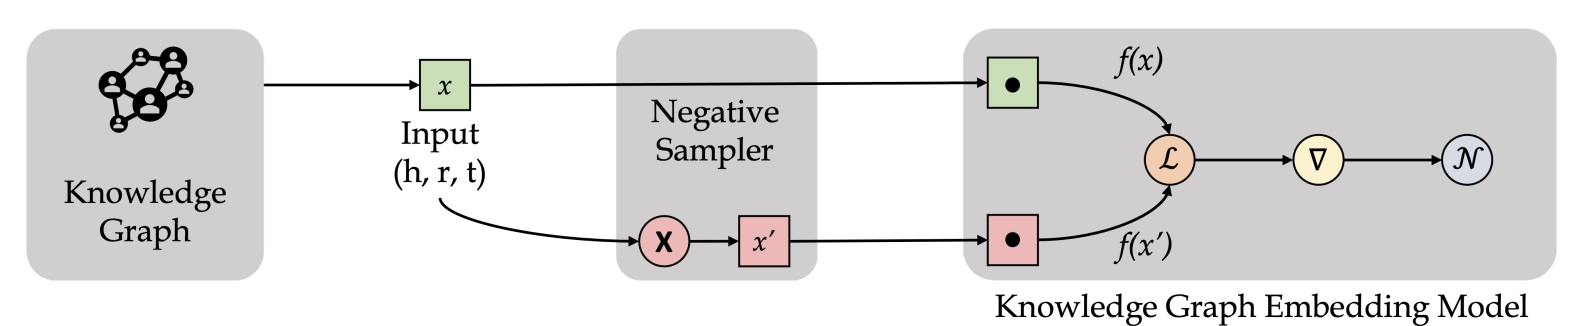
\includegraphics[width=0.8\textwidth]{NS.png} % Adjust the width to 80% of the text width
  \caption{General Structure of Random Negative Sampling Methods, figure taken from \textcite{madushanka2024negative}} % Caption for the figure
  \label{fig:NS} % Label for referencing this figure
\end{figure}

Variants of Static Random Negative Sampling: 
\begin{itemize}
    \item \textbf{Uniform Negative Sampling:} This method involves substituting either the head or the tail entity of a positive triplet with an entity randomly selected from the entity set using a uniform distribution. Despite its simplicity, it sometimes generates false negatives, highlighting its limitations in recognizing semantic relationships.
    \item \textbf{Random Corrupt Negative Sampling:} An extension of uniform negative sampling that also includes the corruption of the relation of the positive triple, enhancing the representation of relational information.
    \item \textbf{Batch NS:} A novel strategy that promotes the reuse of samples within the same mini-batch to serve as negative candidates. This method expands upon the conventional uniform sampling technique and introduces an efficient way to manage resources.
\end{itemize}


\section{EmbedKGQA: The Question Answering Pipeline}

This section is citing the from of \textcite{saxena-etal-2020-improving}.

\begin{figure}[!ht] % 'h!' places the figure here, within your text
  \centering % Centers the figure
  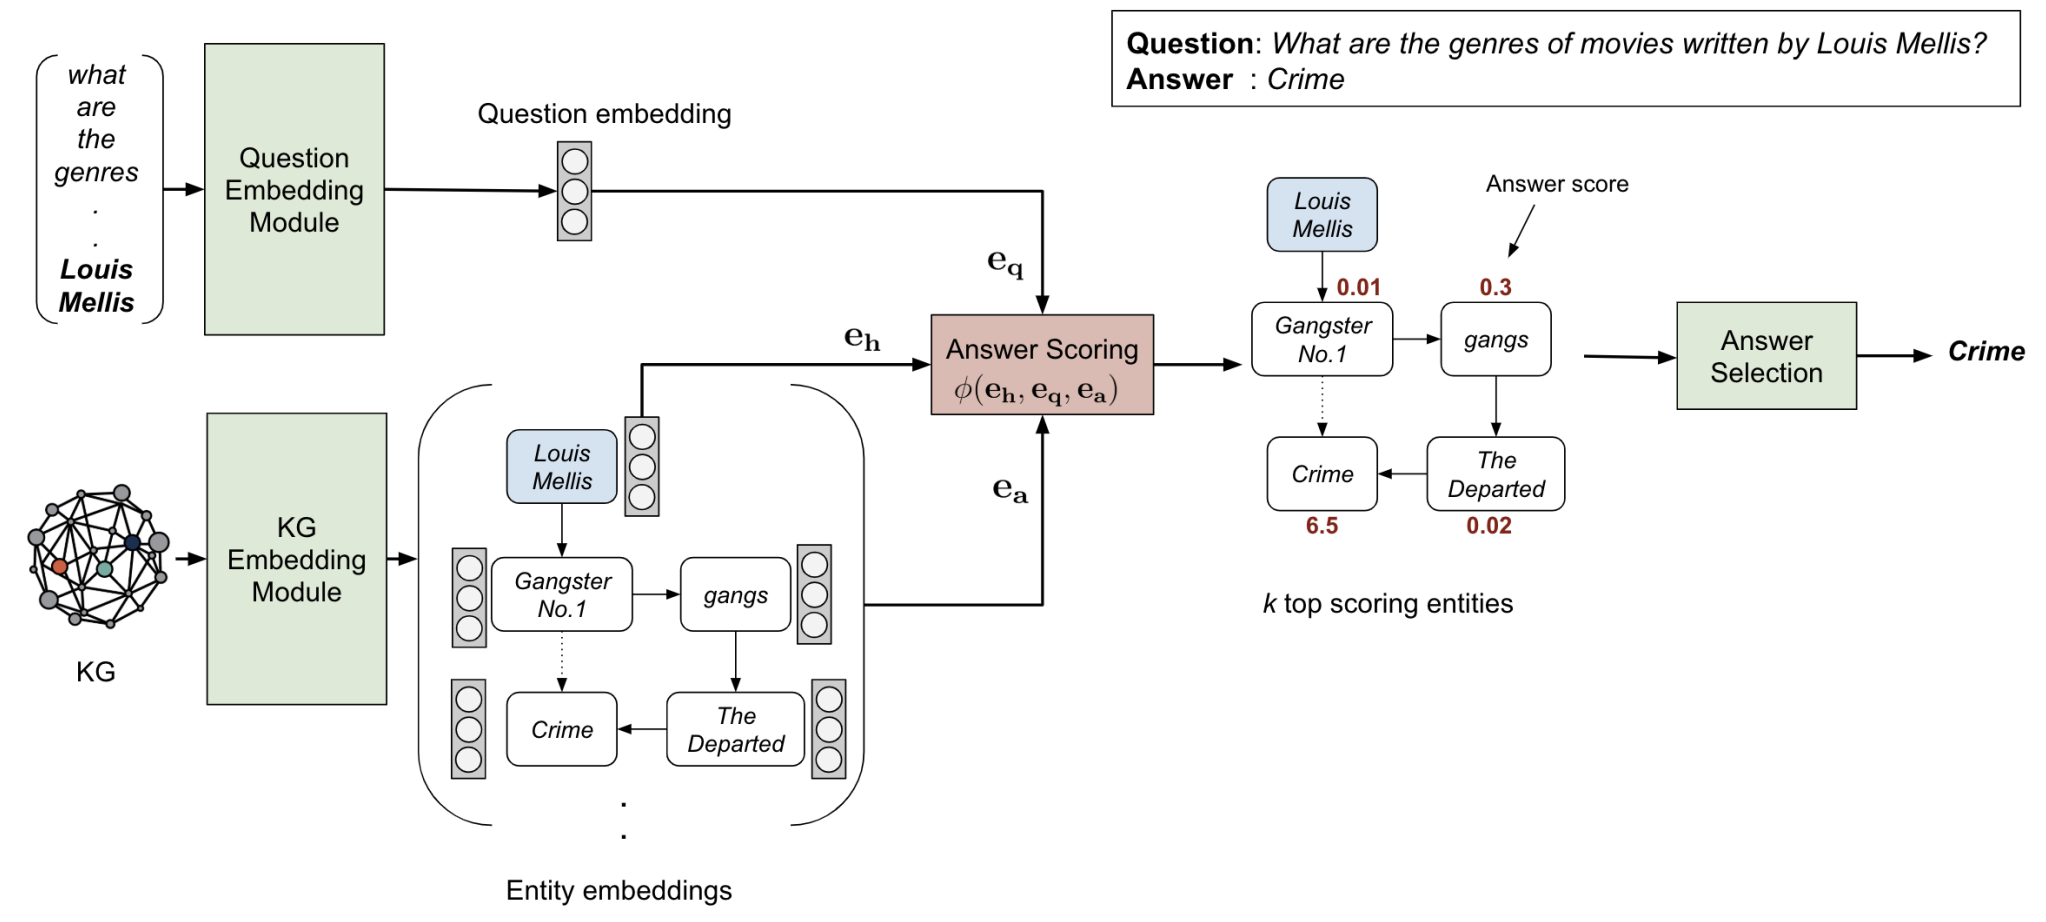
\includegraphics[width=0.9\textwidth]{EmbedKGQA.png} % Adjust the width to 80% of the text width
  \caption{Overview of EmbedKGQA taken from \textcite{saxena-etal-2020-improving}} % Caption for the figure
  \label{fig:EmbedKGQA} % Label for referencing this figure
\end{figure}

EmbedKGQA is a sophisticated method designed to answer complex questions using knowledge graphs (KGs). The process consists of three modules: KG Embedding Module, Question Embedding Module, and Answer Selection Module.

\subsection{KG Embedding Module}
The KG Embedding Module is foundational in EmbedKGQA, where it transforms entities and relations from a knowledge graph into high-dimensional vector spaces using embedding techniques like ComplEx and DistMult. The transformation of entities and relations into embeddings involves several key aspects:
\begin{itemize}
    \item \textbf{Intricate Relationships:} In a knowledge graph, the relationships between entities can be highly detailed and multifaceted. Embeddings capture these intricacies by representing both the direct and indirect connections that an entity may have with others within the graph.

    \item \textbf{Attributes:} Attributes of entities, such as categories, properties, and other descriptive markers, are encoded into the embeddings. This ensures that the vector representation contains comprehensive information that characterizes each entity uniquely.
    \item \textbf{Types:} Different types of entities and relations (like 'person', 'organization', 'location' for entities, or 'works\_for', 'located\_in' for relations) are also integrated into the embeddings. This allows the model to understand and differentiate the roles and functionalities of various entities and relations within the graph.
    \item \textbf{ComplEx Embeddings:} ComplEx embeddings represent entities and relations in complex vector spaces, allowing for the capture of rich, latent structures within the data. This capability is crucial for modeling complex relationships within the KG, enhancing the system's ability to handle multifaceted queries effectively.
    \item \textbf{DistMult Embedding:} DistMult simplifies the embedding process by using real-valued vectors instead of complex numbers. This function evaluates the interaction of entities and relations through a simple dot product, emphasizing efficient computation and straightforward interpretation of embeddings. DistMult is particularly effective for modeling symmetric relationships in the knowledge graph.
\end{itemize}
Through this embedding process, complex, multi-dimensional data is converted into a uniform format (vectors), which machines can efficiently process for various tasks like similarity assessment, relation prediction, and question answering. This vectorized form preserves the semantic richness of the original data, making it actionable for AI applications.


\subsection{Question Embedding Module}
The Question Embedding Module in EmbedKGQA handles the conversion of natural language questions into a format that can be compared with the embedded entities and relations of the knowledge graph. This process typically involves several steps:
\begin{itemize}
    \item \textbf{Initial Embedding:} A pre-trained language model like RoBERTa is used to transform the text of the question into an initial high-dimensional vector (768 dimensions). This vector captures the syntactic and semantic nuances of the question.
    \item \textbf{Feedforward Neural Network:} The initial vector is then passed through four fully connected linear layers with ReLU activation. These layers serve to refine and adapt the vector, ensuring it aligns well with the dimensions and characteristics of the KG embeddings.
    \item \textbf{Projection into Complex Space:} Finally, the output from the feedforward network is projected into the same complex vector space as the KG embeddings. This ensures that the question embeddings can be directly compared with entity and relation embeddings using the scoring function in subsequent processes.
\end{itemize}

\subsection{Scoring Function}
The scoring function $\phi$ used in EmbedKGQA, particularly with ComplEx or DistMult models, quantitatively assesses how well a given triplet (head entity, relation, tail entity) aligns with the factual data encoded in the knowledge graph. For ComplEx, the scoring function can be expressed as:
\[
\phi(h, r, t) = \text{Re}(\mathbf{e}_h \cdot \mathbf{e}_r \cdot \overline{\mathbf{e}_t})
\]
Here, $\text{Re}$ denotes the real part of the complex product, $\mathbf{e}_h$, $\mathbf{e}_r$, and $\mathbf{e}_t$ are the complex embeddings of the head, relation, and tail entities respectively, and $\overline{\mathbf{e}_t}$ is the conjugate of the tail entity embedding.

For DistMult, the function simplifies as it only involves real-valued embeddings:
\[
\phi(h, r, t) = \mathbf{e}_h \cdot \mathbf{e}_r \cdot \mathbf{e}_t
\]
This dot product directly gives the score, representing the compatibility of the triplet without considering complex numbers.

Both functions aim to maximize the score for true triplets and minimize it for false ones, guiding the training process in refining embeddings to better represent the underlying structure of the knowledge graph.


\section{Experiment}
\subsection{Dataset}
\sloppy
In our exploration of KGQA capabilities, we engaged with the MetaQA \parencite[]{zhang2017variational} dataset, a substantial multi-hop KGQA dataset tailored for the movie domain. The dataset is composed of an extensive collection of questions, exceeding 400k in number, and is categorized by the complexity of the information retrieval required—encompassing 1-hop, 2-hop, and 3-hop questions, however in our case we have just tested for 1-hop questions-answering data set. These questions are intricately connected to a movie knowledge graph, rich with entities including actors, directors, and genres, providing a robust framework for performance evaluation. 
\sloppy
For the purposes of our experiments, we selected the "ntm" version of the questions, focusing on the essence of the queries to examine our system’s core answering capabilities. Accompanying the QA data, the MetaQA dataset incorporates a knowledge graph with approximately 135k triples, 43k entities, and nine distinct relations. This comprehensive assembly enables a thorough assessment of KGQA systems, specifically examining their proficiency in handling queries that require an ascending degree of deductive reasoning and inferential capacity.

\subsection{Benchmarking with Classical Method: Cosine Similarity}
This section is citing \textcite{ganesan2024automated}.

Our primary approach to benchmarking involves the use of cosine similarity to measure the effectiveness of the EmbedKGQA system. Cosine similarity is a metric used to determine how similar two vectors are, typically in a high-dimensional space. It calculates the cosine of the angle between the two vectors, with a smaller angle indicating higher similarity. Essentially, it assesses whether two vectors are oriented in the same direction. This measure is widely applied in text analysis, especially for gauging the similarity between documents.

This method involves the following steps:

\begin{itemize}
    \item \textbf{Vectorization:} First, we transform both the question and the candidate answers into vector representations using the embedding techniques described in the KG and Question Embedding Modules of our system.
    \item \textbf{Cosine Similarity Calculation:} We then calculate the cosine similarity between the question vector and each candidate answer vector. This metric measures the cosine of the angle between two vectors, providing a value between -1 and 1 where 1 indicates identical directions, 0 indicates orthogonality, and -1 indicates opposite directions.
    \item \textbf{Answer Selection:} The candidate answer with the highest cosine similarity score is selected as the most probable answer to the question. This process is repeated across a comprehensive set of questions to evaluate the overall effectiveness of the model.
\end{itemize}

\subsection{Research Design}

In this study, we initiate the experimental framework by generating Knowledge Graph Embeddings (KGEs) using two distinct embedding models, namely ComplEx and DistMult. These embeddings are critical in exploring their integral role within Knowledge Graph Question Answering (KGQA) systems. KGQA systems are designed to enable intuitive interactions with structured knowledge bases by processing natural language queries. The effectiveness of these systems significantly depends on the robustness of the KGEs, which capture the semantic relationships between entities.

To investigate the influence of various negative sampling techniques on the efficacy of these KGE models, we apply different strategies including Uniform, Random Corrupt, and Batch Negative Sampling. We generate three variations of KGEs for each embedding model, corresponding to these negative sampling methods, resulting in six distinct sets of KGEs, outlined as follows:

\begin{enumerate}
\item ComplEx with Uniform Negative Sampling
\item ComplEx with Random Corrupt Negative Sampling
\item ComplEx with Batch Negative Sampling
\item DistMult with Uniform Negative Sampling
\item DistMult with Random Corrupt Negative Sampling
\item DistMult with Batch Negative Sampling
\end{enumerate}

Following the generation of these embeddings, we freeze them to proceed with the subsequent stages of the KGQA pipeline. Within the Embed-KGQA pipeline, we employ two different approaches for question embeddings: RoBERTa and SentenceTransformer. These approaches facilitate the mapping of questions to their corresponding entities in the knowledge graph by integrating the question embeddings with the frozen KGEs.

Subsequently, the Answer Selection Module is activated, which employs the previously generated and frozen KGEs in combination with the question embeddings. For each query, the system calculates compatibility scores between the question embeddings and potential answer entity embeddings from the knowledge graph using a predefined scoring function. This function assesses both the semantic proximity and structural data present in the KGEs. The model determines the most suitable answer based on the highest compatibility score, thereby striving to provide accurate and efficient responses to the queries.

Thus, the method encompasses 12 variations of the Embed-KGQA pipeline by combining the six types of KGEs with the two question embedding options. Evaluation metrics such as accuracy,and hits@k are utilized to provide a comprehensive assessment of model performances across the different configurations. Additionally, we conduct a comparative analysis against a baseline cosine - similarity algorithm to see which gives a higher percentage of questions correctly answered.

\section{Results}

\subsection{Performance of KGEs with varying Negative Sampling Techniques}

For comparing performance the six variations of KGEs we use the following three metrics for the test set:
\begin{itemize}
    \item \textbf{Mean Rank:} \textcite{bordes2013translating} defines \textit{Mean Rank} as the average position of the true entity in a ranked list of candidate entities. The metric is calculated by averaging the ranks assigned to the correct entity across all validation queries, and is formally expressed as:

\[
\text{Mean Rank} = \frac{1}{|Q|} \sum_{i=1}^{|Q|} \text{rank}_i
\]

where \( |Q| \) represents the number of queries in the validation set, and \( \text{rank}_i \) is the rank of the correct entity for the \(i\)-th query. The rank is determined by ordering all candidate entities by descending score, with a rank of 1 denoting the top position. A lower Mean Rank indicates a model's effectiveness in ranking true entities closer to the top of the list, reflecting higher predictive accuracy. Conversely, a higher Mean Rank suggests the model often ranks correct entities lower, indicating reduced performance.
 
    \item \textbf{Mean Reciprocal Rank(MRR):}  \textcite{yang2015embedding} defines \textit{Mean Reciprocal Rank} (MRR) as a statistical measure used to evaluate the performance of models in ranking correct entities within a list of predictions. The metric is calculated by taking the reciprocal of the ranks assigned to the correct entity across all validation queries and then averaging these values. The formal expression for MRR is:

\[
\text{MRR} = \frac{1}{|Q|} \sum_{i=1}^{|Q|} \frac{1}{\text{rank}_i}
\]

where \( |Q| \) is the number of queries in the validation set, and \( \text{rank}_i \) denotes the rank of the correct entity for the \(i\)-th query, with ranks ordered such that a rank of 1 corresponds to the top position. A higher MRR value indicates that the model frequently places the correct entities near the top of the list, demonstrating a higher level of accuracy in predictions. Conversely, a lower MRR suggests that the correct answers are ranked lower on average, indicating poorer performance.

    \item \textbf{Hits@k:} \textcite{yang2015embedding} defines \textit{Hits@k} as a performance metric used to evaluate the effectiveness of models in retrieving relevant entities within the top \( k \) positions of a ranked list. The metric is calculated by determining the percentage of queries for which the correct entity appears in the top \( k \) ranks across all validation queries. The formal expression for Hits@k is:

\begin{align*}
\text{Hits@k} = & \frac{\text{Number of queries where the correct entity}}{|Q|} \\
& \times \text{ is ranked within the top } k \times 100
\end{align*}


where \( |Q| \) represents the total number of queries in the validation set. A higher Hits@k percentage indicates that the model is more effective at ranking the correct entities within the top \( k \) positions, suggesting better retrieval performance. Conversely, a lower Hits@k score indicates that the model struggles to rank correct entities in the top ranks, pointing to potential areas for improvement in the model's ranking capabilities.

\end{itemize}

\begin{table}[htbp]
\centering
\caption{Evaluation Metrics for Different Sampling and Embedding Methods}
\label{tab:evaluation_metrics}
\begin{tabular}{@{}lllll@{}}
\toprule
KGE & Sampling & Mean Rank & MRR & Hits@10 \\
\midrule
\multirow{3}{*}{ComplEx} & Uniform & 397.48 & 0.2742 & 0.3664 \\
 & Random Corrupt & \textbf{357.62} & \textbf{0.2849} & \textbf{0.3886} \\
 & Batch NS & 463.07 & 0.2668 & 0.3459 \\
\midrule
\multirow{3}{*}{DistMult} & Uniform & 528.17 & 0.2386 & 0.3360 \\
 & Random Corrupt & 477.78 & 0.2554 & 0.3400 \\
 & Batch NS & 660.01 & 0.1922 &  0.2756 \\
\bottomrule
\end{tabular}
\end{table}

\paragraph{}From this we can see that an overall pattern emerges. Overall, ComplEx performs better than DistMult and Random Corrupt does better than Batch NS and Random Uniform. So, the best performing KGE is ComplEx embeddings with Random Corrupt Negative Sampling. 

\paragraph{}This can be justified as it is only in Random Corrupt Negative Sampling that the head or the tail entity gets replaced along with the relation. In-case of both Random Uniform and Batch NS only the head or the tail entity gets replaced. So, it would make sense for Random Corrupt Negative sampling to have less accidental negative triplets that might be factually true. 

\paragraph{}The superior performance of ComplEx over DistMult can be largely attributed to its enhanced ability to model a broader spectrum of relation types in knowledge graphs, particularly antisymmetric and inverse relations. DistMult, constrained by its use of symmetric scoring functions, assigns identical scores to both \((h, r, t)\) and \((t, r, h)\), rendering it incapable of distinguishing between certain types of relational structures. This limitation notably affects its ability to accurately represent antisymmetric relations, where the directional aspect of the relation is crucial. 

\paragraph{}ComplEx, by contrast, introduces an additional degree of freedom through the use of complex-valued embeddings. The imaginary components of these embeddings allow ComplEx to effectively capture antisymmetric relations by varying the sign of the score depending on the order of the head and tail entities. Specifically, if \(\text{Im}(r) \neq 0\), the scoring function of ComplEx, \(\text{Re}(\langle h, r, \overline{t} \rangle)\), will yield different values when the positions of \(h\) and \(t\) are switched, thus successfully modeling the antisymmetry.

\paragraph{}Moreover, ComplEx's ability to model inverse relations enhances its robustness. It can differentiate between relations and their inverses by treating one relation's embedding as the conjugate of the other, allowing it to maintain accurate relation-specific projections in the embedding space. This is a significant advantage over DistMult, where the commutative property of multiplication in its scoring function fails to differentiate between a relation and its inverse, potentially conflating distinct relational meanings and affecting the model's overall predictive accuracy. 

\subsection{Question Answering Pipeline Performance}

For comparing performance the twelve variations of Embed-KGQA we use the following two metrics for the test set:
\begin{itemize}
    \item \text{Accuracy}
    \item \text{Hits@5}
    \item \text{Hits@10}
\end{itemize}
\sloppy
\begin{table}[htbp]
\centering
\footnotesize % Makes the text of the table smaller
\caption{Evaluation Metrics for Different Question Answering Pipeline Performances}
\label{tab:evaluation_metrics1}
\begin{tabular}{@{}llllll@{}}
\toprule
Question Encoder & KGE & Sampling & Accuracy & Hits@5 & Hits@10 \\
\midrule
\multirow{6}{*}{RoBERTa} & \multirow{3}{*}{ComplEx} & Uniform & 0.357495 & 0.791998  & 0.965316\\
                         &                          & Random Corrupt & \textbf{0.392279} & \textbf{0.824068} & \textbf{0.967327}\\
                         &                          & Batch NS & 0.346570 & 0.761978  & 0.916406\\
\cline{2-6} % This adds a horizontal line from the second to the sixth column
                         & \multirow{3}{*}{DistMult} & Uniform &  0.264101 & 0.606211 & 0.808269\\ 
                         &                          & Random Corrupt &  0.287351 & 0.596211 & 0.798269\\ 
                         &                          & Batch NS & 0.224916 & 0.555009 & 0.729066\\
\midrule
\multirow{6}{*}{SentenceTransformer} & \multirow{3}{*}{ComplEx} & Uniform & 0.274033 & 0.565004& 0.719332\\
                         &                          & Random Corrupt & 0.277615 & 0.594501 & 0.722047\\
                         &                          & Batch NS & 0.262626 & 0.556406 & 0.699058\\
\cline{2-6} % This adds a horizontal line from the second to the sixth column
                         & \multirow{3}{*}{DistMult} & Uniform & 0.141218&0.398723&0.527073\\
                         &                          & Random Corrupt  & 0.175541&0.445541&0.623555\\
                         &                          & Batch NS & 0.139007 & 0.396813& 0.527576\\
\bottomrule
\end{tabular}
\end{table}
\sloppy

From this table we can clearly see that RoBERTa is clearly a better as a Question Encoder than SentenceTransformer. Moreover, ComplEx embeddings perform better than DistMult which is in line with our previous findings. Also, overall Random Corrupt is the best performing Negative Sampling Techniques followed by Random Uniform and Batch NS.
Hence, our best model is used ComplEx Embeddings with Random Corrupt Negative Sampling for KGE Computation and RoBERTa as for Question Embeddings. In the follwing section we compare our benchmark model with our best performing model.

\subsection{Comparison of Cosine Similarity and EmbedKGQA}
We assessed the performance of both methods by their ability to correctly answer a set of 9,992 questions. A correct answer was marked with a '1', while an incorrect one was marked with a '0'. The results are as follows:
\begin{itemize}
    \item \textbf{Cosine Similarity:} Out of 9,992 questions, the cosine similarity approach correctly answered 573, yielding a success rate of approximately 5.73\%.
    \item \textbf{EmbedKGQA:} The best performing EmbedKGQA pipeline correctly answered 3,919 out of 9,992 questions, resulting in a significantly higher success rate of approximately 39.23\%.
\end{itemize}

The disparity in performance is notable, with the EmbedKGQA pipeline outperforming the cosine similarity approach by around 30.39\% points in terms of the proportion of correctly answered questions. This substantial difference underscores the effectiveness of specialized methods like EmbedKGQA for the task at hand.
\
It is evident from the results that EmbedKGQA benefits from its tailored architecture which is optimized for understanding and leveraging the structured nature of knowledge graphs, leading to a more profound comprehension of the relationships between entities and consequently, a higher accuracy in the question answering task.
\
The marked difference in performance between the two methods suggests that while cosine similarity provides a baseline for semantic matching, it lacks the nuanced understanding of knowledge graph structure that is encoded into the EmbedKGQA pipeline. This finding aligns with the inherent limitations of cosine similarity when applied to complex relational queries, as it may not fully capture the multi-dimensional relationships present within a knowledge graph.
\
The EmbedKGQA's advantage likely arises from its ability to integrate relational context into its embeddings, offering a more refined approach to question answering that considers the inter-connectivity of entities within the graph.

\section{Conclusion}

This study has systematically explored the influence of various negative sampling techniques on the effectiveness of Knowledge Graph Embeddings (KGEs) within Knowledge Graph Question Answering (KGQA) systems. Our results indicate that the ComplEx model, coupled with Random Corrupt Negative Sampling, delivers the most robust performance across multiple metrics including Mean Rank, Mean Reciprocal Rank (MRR), and Hits@k. This configuration not only enhances the quality of embeddings but also significantly improves the downstream KGQA performance by effectively capturing complex relational patterns inherent in knowledge graphs.

The integration of sophisticated question embedding techniques such as RoBERTa within the EmbedKGQA pipeline further underscores the critical role of advanced natural language processing models in improving the accuracy and efficiency of KGQA systems. These findings highlight the pivotal interplay between the choice of negative sampling strategies and the selection of embedding models in optimizing KGQA frameworks.

\subsection{Future Research Directions}

Despite the advancements demonstrated in this study, several avenues remain open for future research:
\begin{itemize}
  \item \textbf{Dynamic Adaptation of Embeddings:} Future work could explore the development of adaptive KGE models that dynamically update embeddings in response to new information or evolving data within knowledge graphs. This would be particularly beneficial for KGQA systems deployed in rapidly changing domains.
  \item \textbf{Incorporation of Multimodal Data:} Integrating multimodal data sources, such as images and videos, into KGQA systems could enhance the richness of the answers provided and expand the types of queries these systems can address.
  \item \textbf{Cross-Lingual KGQA:} Investigating the efficacy of KGQA systems across different languages and cultural contexts would be invaluable, especially for global applications. This involves enhancing the understanding of cross-lingual entity recognition and linking in knowledge graphs.
  \item \textbf{Explainability and Trust:} Developing methodologies to improve the explainability of KGQA systems would help in building trust and facilitating broader adoption, particularly in critical areas such as healthcare and finance.
\end{itemize}

These directions not only promise to expand the capabilities of KGQA systems but also aim to address the growing need for personalized, context-aware information retrieval and decision-making systems.

\printbibliography
\end{document}